% ISCB abstract-book single-page, print-ready PDF.
% Specs: US Letter; margins top 0.75in, left/right/bottom 0.5in; two columns, 0.25in gap;
% 11pt Times; title 14-16pt bold centered; presenting author starred. Print-ready, no reformatting applied.
\documentclass[11pt,twocolumn,letterpaper]{article}
\usepackage[T1]{fontenc}
\usepackage{mathptmx}        % Times New Roman-like serif for text and math
\usepackage[letterpaper,top=0.75in,left=0.5in,right=0.5in,bottom=0.5in]{geometry}
\usepackage{graphicx}
\usepackage{caption}
\usepackage{makecell}
\usepackage{booktabs}
\usepackage{microtype}
\setlength{\columnsep}{0.25in}
\captionsetup{font=small,labelfont=bf,skip=4pt}
\setlength{\parindent}{1em}
\setlength{\parskip}{0pt}
\pagestyle{empty}

\begin{document}

\twocolumn[
  \begin{center}
    {\fontsize{15}{17}\selectfont\bfseries
     Recovering and Redirecting Peptide Backbone Conformation via\\
     Contact-Conditioned C$\alpha$ Generation in a Cross-Reactive pMHC/TCR System\par}
    \vspace{5pt}
    {\normalsize Authors$^{*}$\par}
    \vspace{8pt}
  \end{center}
]

\noindent\textbf{Motivation.}
Cross-reactive TCR/pMHC systems, in which one receptor engages chemically distinct peptides through
distinct bound backbone conformations, pose a question orthogonal to conventional epitope design.
Can a structure-conditioned generative model be steered, from receptor-side information alone, toward a
specific target backbone conformation, including, deliberately, one other than the conformation nearest its
conditioning input? We use a minimal two-state system: the DMF5 TCR on HLA-A*02:01, which accommodates two
decameric peptides, GIG (\texttt{SMLGIGIVPV}, crystal 6AM5) and DRG (\texttt{MMWDRGLGMM}, 6AMU), via
backbones separated by 2.87\,\AA{} C$\alpha$ RMSD. That difference is almost entirely C-terminal (P1 to P4
are identical to within 1.14\,\AA{}, while P6 diverges by 5.62\,\AA), and register is defined by which
peptide position buries in the F-pocket (p10 for GIG, p9 for DRG).

\noindent\textbf{Methods.}
Conditioning only on receptor-side contact residues, with no peptide-backbone template, we asked whether
RFdiffusion can generate a C$\alpha$ backbone that recovers a peptide's own native register or crosses into
the alternate one. We generated a converged corpus of \textbf{24{,}831} designs: 600 designs per crystal for
each of 20 conditioning schemes, plus a focused N-terminus-seeding experiment. Designs are scored against a
three-criterion register test calibrated not to a single crystal but to \textbf{native molecular-dynamics
ensembles} (Amber ff19SB, TIP3P, physiological \textbf{310\,K}, 50\,ns): C$\alpha$ proximity within a
moving-block-bootstrap acceptance band (DRG within 1.48\,\AA, 95\% CI 1.36 to 1.58), correct F-pocket
occupant identity, and native burial depth. We additionally correct for a forward/reverse backbone-threading
artifact that raw RMSD cannot detect.

\noindent\textbf{Results.}
Both recovery and redirection are achievable but rare, and are gated by the breadth of conditioning rather
than by any specific curated residue set. Across the de novo corpus, 7 of 16{,}919 designs recover the
native DRG register (best 1.07\,\AA) and 4 of 16{,}919 cross into the alternate DRG register (best
1.44\,\AA), every hit forward-threaded and seating the correct p9 anchor, all arising from the broadest
conditioning schemes. Critically, our no-conditioning control produced \textbf{zero} designs that dock in
the groove or come close in RMSD to either native backbone: \textbf{0 of 1{,}533} unconditioned draws
entered the acceptance band or seated an anchor, so the recovery and crossing events are real signal above a
true zero-information background, not sampling noise. A templating control that supplies backbone geometry
directly recovers register almost at will and monotonically with the number of templated residues, whereas
contact conditioning alone only weakly determines it, locating register in a spatially confined C-terminal
signal. These results, from a single well-characterized system, map the current capability boundary of
contact-conditioned backbone generation and separate what it can retrieve from what must still be supplied
as explicit geometry.

\vspace{2pt}
\begin{center}
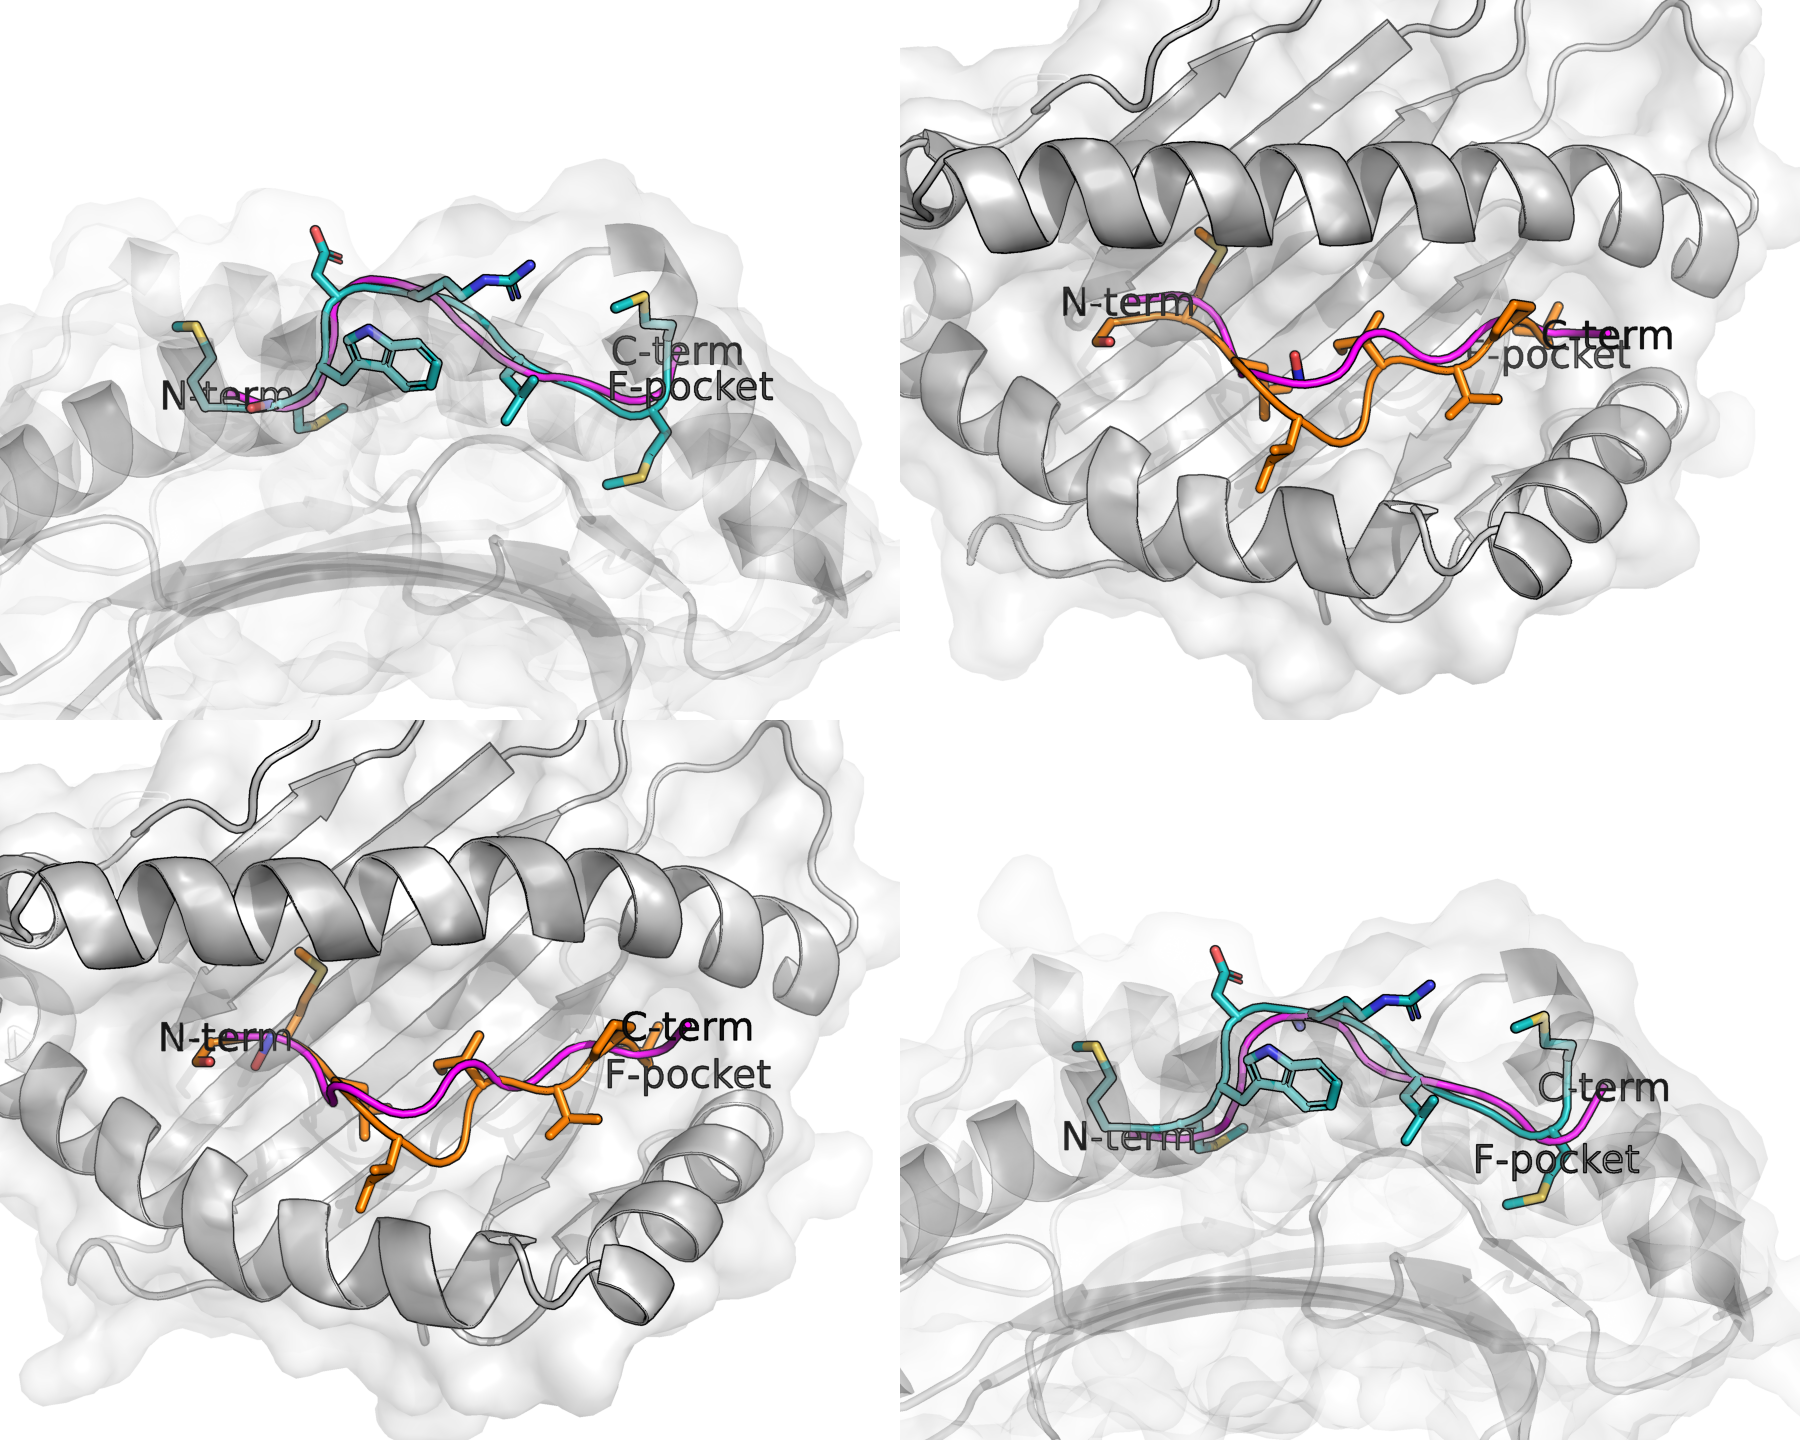
\includegraphics[width=\columnwidth]{../figures/fig2_recovery_crossing/fig2_recovery_crossing.png}
\end{center}
\vspace{-2pt}

{\small
\captionof{table}{Full converged corpus (24{,}831 designs), scored against the 310\,K native envelope.
Recoveries land in the peptide's own native register; crossings land in the alternate register.}
\renewcommand{\arraystretch}{1.35}
\setlength{\tabcolsep}{5pt}
\begin{tabular}{@{}lrccc@{}}
\toprule
design group & $n$ & \makecell{best RMSD\\to own (\AA)} & recov. & cross. \\
\midrule
de novo (receptor contacts only)   & 16{,}919 & 1.07 & 7      & 4  \\
null control (no conditioning)      & 1{,}533  & 2.05 & 0      & 0  \\
templated (native backbone given)   & 6{,}041  & 0.10 & 1{,}282 & 1  \\
crossover (N-terminus given)        & 338      & 0.54 & 16     & 20 \\
\bottomrule
\end{tabular}\par
}

\vspace{3pt}
\noindent\textbf{Availability.}
Code, the MD-calibrated scorer, campaign drivers, and curated design archives:
\texttt{github.com/sermare/if-mhc}.

\end{document}
